%\documentclass[11pt,a4paper]{memoir}
\documentclass[11pt,a4paper]{article}
%\documentclass[11pt,a4paper]{scrartcl}
\usepackage[table]{xcolor}
%\usepackage{colortbl}
\usepackage{pgfplots}
\usepackage[british,UKenglish,USenglish,english,american]{babel}
%\usepackage[a4paper, total={16cm, 23cm}]{geometry}
\usepackage[tmargin = 1.25in,bmargin = 1.25in,lmargin = 1in,rmargin = 1in]{geometry}
\usepackage{tikz}
\usepackage{graphicx}
\usepackage{chemmacros}
\usepackage{chemfig}
%\usepackage{ghsystem}
\usechemmodule{redox}
%\usepackage{chemnum}
%\usepackage{bohr}
%\usepackage{elements}
%\usepackage{endiagram}
%\usepackage{modiagram}
%\usepackage{chemgreek}
\usepackage{mhchem}
\usepackage{enumitem}
\usepackage{makeidx}
\usepackage{epstopdf}
\usepackage{amssymb}
\usepackage{mathrsfs}
%\usepackage{minted}
\usepackage{amsmath}
\usepackage{enumitem}
\usepackage[english]{varioref}
\usepackage[english]{babel}
\usepackage{lipsum}
\usepackage{fancyhdr}
\pagestyle{fancy} 
\usepackage{float}
\usepackage{empheq}
\usepackage[framemethod=tikz]{mdframed}
\usepackage{epstopdf}
\numberwithin{equation}{section}
\usepackage{eso-pic}
\usepackage{calc}
\usepackage{nccmath}
\usepackage{caption}
\usepackage{subcaption}
\usepackage{gensymb}
\usepackage{amsfonts,amsthm,epsfig,epstopdf,titling,url,array}
\usepackage{siunitx}
\usepackage{xcolor}
\usepackage{multicol}
\usepackage{boondox-cal}
%\usepackage{paralist}




\DeclareSIUnit\atm{atm}

\fancypagestyle{firstpage}{
	\rhead{\begin{picture}(0,0) \put(-30,0){
\includegraphics[width=1cm]{figures/MCI_4C_bw.eps}} \end{picture}}
}
\fancyhead[L]{\slshape\nouppercase{\leftmark}}
\chead{}
\rhead{\begin{picture}(0,0) \put(-30,0){
\includegraphics[width=1cm]{figures/MCI_4C_bw.eps}} \end{picture}}
\lfoot{\textit{}}
\cfoot{-\ \thepage\ -}
\rfoot{\textit{}}
\renewcommand{\headrulewidth}{0.4pt}
\renewcommand{\footrulewidth}{0.4pt}
\newcommand{\abs}[1]{\left|#1\right|}
\definecolor{mycolor1}{rgb}{0.95, 0.95, 0.95}
\definecolor{mycolor2}{rgb}{0.95, 0.95, 0.95}
\definecolor{tableShade}{gray}{0.9}
\newcommand{\sign}{\text{sign}}
\newcommand{\centered}[1]{\begin{tabular}{@{}l@{}} #1 \end{tabular}}
\theoremstyle{it}
\newtheorem{defn}{Definition}[section]
\newtheorem{thm}{Theorem}[section]
\theoremstyle{definition}
\newtheorem{example}{Example}[section]

\newenvironment{myitemize_1}
	{ \begin{itemize}[topsep=0pt]
		\setlength{\topsep}{2pt}		
		\setlength{\itemsep}{2pt}
		\setlength{\parskip}{2pt}
		\setlength{\parsep}{2pt}     }
	{ \end{itemize}                  }


\newmdenv[innerlinewidth=0.5pt, roundcorner=4pt, backgroundcolor = {mycolor1}, linecolor = {mycolor1}, innerleftmargin=6pt,
innerrightmargin=6pt,innertopmargin=6pt,innerbottommargin=6pt]{mybox}

\title{\textbf{Generic Flexible Shaft \\ and Gear-Shaft}}
\author{\textbf{DTL}}

\begin{document}
	\thispagestyle{firstpage}
	\begin{mybox}
		\maketitle
		\vspace{125mm}
	\end{mybox}
	\newpage
	\tableofcontents
	\listoffigures	
	\listoftables
	\newpage

{In this document the model of a generic flexible shaft is derived.}


\section{Equivalent mathematical model}
The mass-spring-mass model is a valid approximation of the flexible shaft and it will be used to modelize it and its extrapolation to a generic simplified gear.
Figure \ref{figure_cranckshaft} shows a generic flexible shaft where $\tau_m$ 
is the torque actuated by a primer mover and $\tau_l$ is assumed to be a disturbance or a generic unknown load 
torque.
\subsection{Model Derivation} 
The model presents two rotational inertia masses ($J_m, J_l$) connected by a torsional spring ($k_{\vartheta}$) which include a friction term ($b_{\vartheta}$). Both two masses are connected to the chassis by two virtual bearings modeled with two simple viscosity coefficients: $b_m$ and $b_l$.

Mathematical model can be derived using Euler-Lagrange equations as follows
\begin{equation}\label{elagrange_1}
	\frac{d}{dt}\left(\frac{\partial E_{kin}}{\partial \dot{q}_1} \right) - 
	\frac{\partial E_{kin}}{\partial q_1} + \frac{\partial E_{pot}}{\partial 
		q_1} =\underbrace{Q_{diss}^{(12)} + Q_1}_\text{not conservative force}
\end{equation}
\begin{equation}\label{elagrange_2}
	\frac{d}{dt}\left(\frac{\partial E_{kin}}{\partial \dot{q}_2} \right) - 
	\frac{\partial E_{kin}}{\partial q_2} + \frac{\partial E_{pot}}{\partial 
		q_2} = \underbrace{Q_{diss}^{(21)} + Q_2}_\text{not conservative force}
\end{equation}
\begin{figure}[H]
	\centering
	\includegraphics[width = 320pt, keepaspectratio] {figures/msm/flexshaft_1.eps}
	\captionsetup{width=0.5\textwidth}		
	\caption{Generic flexible shaft model.}
	\label{figure_cranckshaft}
\end{figure}
Where $Q_1$, $Q_2$, $Q_{diss}^{(12)}$ and $Q_{diss}^{(21)}$ are the generalized 
forces, like magnetic force, unknown load, disturbance and  friction or in general not conservative force\footnote{A conservative force is a force which is derive by a potential and satisfies to the following conditions:
	\begin{flalign}
		\vec{\nabla}\times\vec{f}=\vec{0} &&
	\end{flalign}
	\begin{flalign}
		\oint_{\mathscr{C}}\vec{f}\cdot d\vec{r}=0 &&
	\end{flalign}
	\begin{flalign}
		\vec{f}=-\vec{\nabla}\phi &&
	\end{flalign}
}. 

Applying Eqs.~\eqref{elagrange_1} and~\eqref{elagrange_2} for the case
\begin{equation}
	\begin{aligned}
		q_1&=\vartheta_m \\[6pt]	
		q_2&=\vartheta_l
	\end{aligned}
\end{equation}
The kinematic and potential energy can be written as follows
\begin{equation}
	E_{kin} = \frac{1}{2}J_m\dot{\vartheta}_m^2 + \frac{1}{2}J_l\dot{\vartheta}_l^2
\end{equation}
\begin{equation}
	E_{pot} = \frac{1}{2}k_{\vartheta}\left(\vartheta_m-\vartheta_l\right)^2
\end{equation}

Applying the Lagrange equations we obtain the following motion equations
\begin{flalign}
	J_m\ddot{\vartheta}_m+k_{\vartheta}\left( \vartheta_m-\vartheta_l\right)  &= 
	-b_m\dot{\vartheta}_m-b_{\vartheta}\left(\dot{\vartheta}_m-\dot{\vartheta_l}\right) + 
	\tau_m \\[6pt]
	J_l\ddot{\vartheta}_l-k_{\vartheta}\left( \vartheta_m-\vartheta_l\right)  &= 
	-b_l\dot{\vartheta}_l-b_{\vartheta}\left(\dot{\vartheta_l}-\dot{\vartheta}_m\right) + 
	\tau_l
\end{flalign}
or 
\begin{equation}
	\left\lbrace \begin{aligned}
		\dot{\vartheta}_m &= \omega_m \\[6pt]
		\dot{\omega}_m &= 
		-\frac{k_{\vartheta}}{J_m}\vartheta_m-\frac{b_m+b_{\vartheta}}{J_m}\omega_m 
		+\frac{k_{\vartheta}}{J_m}\vartheta_l+\frac{b_{\vartheta}}{J_m}\omega_l+\frac{1}{J_m}\tau_m
		\\[6pt]
		\dot{\vartheta}_l &= \omega_l \\[6pt]
		\dot{\omega}_l &= 
		\frac{k_{\vartheta}}{J_l}\vartheta_m+\frac{b_{\vartheta}}{J_l}\omega_m-\frac{k_{\vartheta}}{J_l}\vartheta_l-\frac{b_l+b_{\vartheta}}{J_l}\omega_l
		+\frac{1}{J_l}\tau_l
	\end{aligned}\right. 
\end{equation}
The state space representation become
\begin{equation}
	\dot{\vec{z}} = \tilde{\mathbf{G}}\vec{z}+\tilde{\mathbf{H}} \ 
	\tau_m+\tilde{\mathbf{M}} \ \tau_l
\end{equation}
where $\vec{z}=\left[ \begin{matrix}
	\vartheta_m&\omega_m&\vartheta_l&\omega_l
\end{matrix}\right]^T$
and 
\begin{equation}
	\tilde{\mathbf{G}} = 
	\left[ \begin{matrix}
		0&1&0&0\\[6pt]
		-\frac{k_{\vartheta}}{J_m}&-\frac{b_m+b_{\vartheta}}{J_m}&\frac{k_{\vartheta}}{J_m}&\frac{b_{\vartheta}}{J_m}\\[6pt]
		0&0&0&1\\[6pt]
		\frac{k_{\vartheta}}{J_l}&\frac{b_{\vartheta}}{J_l}&-\frac{k_{\vartheta}}{J_l}&-\frac{b_l+b_{\vartheta}}{J_l}
	\end{matrix}\right]
\end{equation}
and $\tilde{\mathbf{H}} =\left[ \begin{matrix}
	0&\frac{1}{J_m}&0&0
\end{matrix}\right]^T$, 
$\tilde{\mathbf{M}} =\left[ \begin{matrix}
	0&0&0&-\frac{1}{J_l}
\end{matrix}\right]^T$.

For our purpose, we want to change the state representation using a new state 
vector 
\begin{equation}
	\vec{x} = \mathbf{T}\vec{z} = \begin{bmatrix} \omega_m \\[6pt] \omega_l \\[6pt] \tau_{\vartheta} \end{bmatrix}
\end{equation}
where\footnote{where 
	\begin{flalign}
		\tau_{\vartheta}=k_\vartheta(\vartheta_m-\vartheta_l) &&
	\end{flalign} 
	which can be written also as 
	\begin{flalign}
		\dot{\tau}_{\vartheta}=k_\vartheta(\omega_m-\omega_l) &&
	\end{flalign} 
	which describes the dynamic of the shaft torsional torque.} $\mathbf{T}$ is 
given by\footnote{the matrix pseudo inverse has been used.}
\begin{equation}
	\mathbf{T} = \left[\begin{matrix}
		0 & 1 & 0 & 0 \\[6pt]
		0 & 0 & 0 & 1 \\[6pt]
		k_{\vartheta} & 0 & -k_{\vartheta} & 0
	\end{matrix}\right]
	\quad \text{and} \quad
	\mathbf{T}^{-1} = \left[\begin{matrix}
		0 & 0 & \frac{1}{2k_{\vartheta}} \\[6pt]
		1 & 0 & 0 \\[6pt]
		0 & 0 & -\frac{1}{2k_{\vartheta}} \\[6pt]
		0 & 1 & 0
	\end{matrix}\right]
\end{equation}
Basically, the linear transformation $\mathbf{T}$ consists in a model reduction. The minimum representation of a dynamical system can be reached applying some matrix analysis results, but also considering the total number of energy storage which are contained into the system. In the case of mass-spring-mass model, we can assume that three components can store energy: the two inertial masses $J_m$ and $J_l$ as kinetic energy, and the torsional spring as potential energy. That means the minimal representation of the mass-spring-mass model is made by three equations.

The new state space representation becomes
\begin{flalign}
	\dot{\vec{z}} &= \tilde{\mathbf{G}}\vec{z}+\tilde{\mathbf{H}} \ 
	\tau_1+\tilde{\mathbf{M}} \ \tau_2 \\[6pt]
	\mathbf{T}^{-1}\dot{\vec{x}} &= 
	\tilde{\mathbf{G}}\mathbf{T}^{-1}\vec{x}+\tilde{\mathbf{H}} \ 
	\tau_1+\tilde{\mathbf{M}} \ \tau_2 \\[6pt]
	%&\vdots \\
	\dot{\vec{x}} &= 
	\mathbf{T}\tilde{\mathbf{G}}\mathbf{T}^{-1}\vec{x}+\mathbf{T}\tilde{\mathbf{H}}
	\ \tau_1+\mathbf{T}\tilde{\mathbf{M}} \ \tau_2
\end{flalign}
or
\begin{mybox}
	\begin{equation}
		\dot{\vec{x}} = \tilde{\mathbf{A}}\vec{x}+\tilde{\mathbf{B}}\,\tau_1+\tilde{\mathbf{E}}\,\tau_2
	\end{equation}
	or
	\begin{equation}\label{two_mass_2}
		\left[ \begin{matrix}
			\dot{\omega}_m \\[6pt]
			\dot{\omega}_l \\[6pt]
			\dot{\tau_{\vartheta}}
		\end{matrix}\right] = 
		\left[ \begin{matrix}
			-\frac{b_m+b_{\vartheta}}{J_m} & \frac{b_{\vartheta}}{J_m} & 
			-\frac{1}{J_m}\\[6pt]
			\frac{b_{\vartheta}}{J_l} & -\frac{b_l+b_{\vartheta}}{J_l} & 
			\frac{1}{J_l}\\[6pt]
			k_{\vartheta} & -k_{\vartheta} & 0
		\end{matrix}\right]
		\left[ \begin{matrix}
			{\omega_m} \\[6pt]
			{\omega_l} \\[6pt]
			{\tau_{\vartheta}}
		\end{matrix}\right] + 
		\left[ \begin{matrix}
			\frac{1}{J_m} \\[6pt]
			0 \\[6pt]
			0
		\end{matrix}\right] \tau_m+
		\left[ \begin{matrix}
			0 \\[6pt]
			\frac{1}{J_l} \\[6pt]
			0
		\end{matrix}\right] \tau_l
	\end{equation}
	where 
	
	\begin{equation*}
		\vec{x} = \left[\begin{matrix} \omega_m&\omega_l&\tau_{\vartheta} 
		\end{matrix} \right]^T
	\end{equation*}
	
	\begin{equation*}
		\tilde{\mathbf{A}} = \mathbf{T}\tilde{\mathbf{G}}\mathbf{T}^{-1} =
		\left[ \begin{matrix}
			-\frac{b_m+b_{\vartheta}}{J_m} & \frac{b_{\vartheta}}{J_m} & 
			-\frac{1}{J_m}\\[6pt]
			\frac{b_{\vartheta}}{J_l} & -\frac{b_l+b_{\vartheta}}{J_l} & 
			\frac{1}{J_l}\\[6pt]
			k_{\vartheta} & -k_{\vartheta} & 0
		\end{matrix}\right]
	\end{equation*}
	
	\begin{equation*}
		\tilde{\mathbf{B}} = \mathbf{T}\tilde{\mathbf{H}} =
		\left[ \begin{matrix}
			\frac{1}{J_m} \\[6pt]
			0 \\[6pt]
			0
		\end{matrix}\right]
		\quad
		\tilde{\mathbf{E}} = \mathbf{T}\tilde{\mathbf{M}} =
		\left[ \begin{matrix}
			0 \\[6pt]
			\frac{1}{J_l} \\[6pt]
			0
		\end{matrix}\right]
	\end{equation*}
	\textbf{Consider the term $\tau_l(t)$ as a disturbance (or load) which perturbs 
		the system.}
	
	\vspace{5mm}
	For a more physical viewpoint the mass-spring-mass (or flexible shaft) dynamic 
	equations can also be written as follows:
	\begin{equation}
		\left\lbrace 
		\begin{aligned}
			& \dot{\omega}_m =\frac{1}{J_m}\Big[ -\big(b_m+b_\vartheta\big)\omega_m+b_{\vartheta}\omega_l - \tau_{\vartheta} + \tau_m\Big] \\[6pt]
			& \dot{\omega}_l = \frac{1}{J_l}\Big[b_\vartheta\omega_m-\big(b_l+b_{\vartheta}\big)\omega_l+ 
			\tau_{\vartheta} + \tau_l\Big] \\[6pt]
			& \dot{\tau}_{\vartheta} = k_{\vartheta}\big(\omega_m-\omega_l\big) 
		\end{aligned}
		\right. 
	\end{equation}
\end{mybox}

\subsection{Natural oscillations}
The frequency of the natural oscillation of the shaft can be evaluated imposing to zero the friction terms and calculating the eigenvalue of the transition matrix, as follows

\noindent setting $b_m=0$,  $b_l=0$ and $b_\vartheta=0$ we obtain the following characteristic polynomial
\begin{equation}\label{eigenvalues_msm}
	\Big|s\mathbf{I}-\tilde{\mathbf{A}}\Big|=\begin{vmatrix}
		s & 0 & 1/J_m \\[6pt]
		0 & s & -1/J_l \\[6pt]
		-k_\vartheta & k_\vartheta & s 
	\end{vmatrix} = s\Big[s^2+k_\vartheta\frac{J_m+J_l}{J_mJ_l}\Big]
\end{equation}
setting $s=j\omega$ to the Eq.~\eqref{eigenvalues_msm} and equating to zero
\begin{equation}
	\omega^2-k_\vartheta\frac{J_m+J_l}{J_mJ_l}=0
\end{equation}
we obtain
\begin{equation}
		\omega_0=\sqrt{k_\vartheta\frac{J_m+J_l}{J_mJ_l}}
\end{equation}
which represent the pulsation of the natural harmonic component of the system.

\section{Extension to a generic gear model}
The mathematical structure of the flexible shaft can be used also to develop a simplified gear.

Let
\begin{equation}
	\omega_l=\omega_m/n_{tg}
\end{equation}
be the relation between driver (m) and follower (l) speeds, where $\omega_l$ is the follower speed and $\omega_m$ is the driver speed. The term $n_{tg}$ represents the ratio between the driver and the follower speeds of the gear.

The mathematical model of the simplified gear is here represented ($b_\vartheta=0$ is assumed), 
\begin{equation}\left\lbrace 
	\begin{aligned}
		\dot{\omega}_m &= \frac{1}{J_m}\Big[\tau_m - \tau_\vartheta^m - b_m\omega_m\Big] \\[8pt]
		\dot{\omega}_l &= \frac{1}{J_l}\Big[\tau_\vartheta^l + \tau_l - b_l\omega_l \Big] \\[8pt]
		\dot{\tau}_\vartheta^m &= k_\vartheta\Big[\omega_m -\omega_l n_{tg} \Big] \\[8pt]
		n_{tg} &= \frac{n_m}{n_l} \\[8pt]
		\tau_\vartheta^m &=\frac{\tau_\vartheta^l}{n_{tg}}
	\end{aligned}\right. 
\end{equation}
where $\tau_\vartheta^m$ is the torsional torque seen at the driver side as well as $\tau_\vartheta^l$ is the torsional torque seen at the follower side, see also Figure~\ref{figure_gear_flexshaft}.
\begin{figure}[H]
	\centering
	\includegraphics[width = 400pt, keepaspectratio] {figures/msm/gear_flexshaft_2.eps}
	\captionsetup{width=0.5\textwidth}		
	\caption{Generic flexible gear-shaft model.}
	\label{figure_gear_flexshaft}
\end{figure}

\section{Flexible Shaft - Model parameters settings}
Parameters setting consist of
\begin{itemize}
	\item[--] $J_m\quad\Big[\SI{}{\kilo\gram\square\meter}\Big]$: Inertia of the \textit{m}-side rotating mass.
	\item[--] $J_l\quad\Big[\SI{}{\kilo\gram\square\meter}\Big]$: Inertia of the \textit{l}-side rotating mass.
	\item[--] $b_m\quad\Big[\SI{}{\newton\second\per\radian}\Big]$: Friction coefficient - \textit{m}-side.
	\item[--] $b_l\quad\Big[\SI{}{\newton\second\per\radian}\Big]$: Friction coefficient - \textit{l}-side.
	\item[--] $k_\vartheta\quad\Big[\SI{}{\newton\per\radian}\Big]$: Internal torsional spring.	
	\item[--] $b_\vartheta\quad\Big[\SI{}{\newton\second\per\radian}\Big]$: Damping of the internal torsional spring.
\end{itemize}

\section{Gear - Model parameters settings}
Parameters setting consist of
\begin{itemize}
	\item[--] $n_m\quad\Big[\SI{}{ad}\Big]$: with $n_l$ forms the gear ratio $n_{tg} = \frac{n_m}{n_l}$.
	\item[--] $n_l\quad\Big[\SI{}{ad}\Big]$: with $n_m$ forms the gear ratio $n_{tg} = \frac{n_m}{n_l}$.
	\item[--] $J_m\quad\Big[\SI{}{\kilo\gram\square\meter}\Big]$: Inertia of the \textit{driver}-side rotating mass.
	\item[--] $J_l\quad\Big[\SI{}{\kilo\gram\square\meter}\Big]$: Inertia of the \textit{follower}-side rotating mass.
	\item[--] $b_m\quad\Big[\SI{}{\newton\second\per\radian}\Big]$: Friction coefficient - \textit{driver}-side.
	\item[--] $b_l\quad\Big[\SI{}{\newton\second\per\radian}\Big]$: Friction coefficient - \textit{follower}-side.
	\item[--] $k_\vartheta\quad\Big[\SI{}{\newton\per\radian}\Big]$: Internal torsional spring.	
\end{itemize}


\end{document} 